\documentclass{article}
%% %\VignetteIndexEntry{MotifDb Overview}
%% %\VignettePackage{MotifDb}
\usepackage[noae]{Sweave}
\usepackage[left=0.5in,top=0.5in,right=0.5in,bottom=0.75in,nohead,nofoot]{geometry}
\usepackage{hyperref}
\usepackage[noae]{Sweave}
\usepackage{color}
\usepackage{graphicx}
\usepackage{caption}
\usepackage{subcaption}

\definecolor{Blue}{rgb}{0,0,0.5}
\definecolor{Green}{rgb}{0,0.5,0}

\RecustomVerbatimEnvironment{Sinput}{Verbatim}{%
  xleftmargin=1em,%
  fontsize=\small,%
  fontshape=sl,%
  formatcom=\color{Blue}%
  }
\RecustomVerbatimEnvironment{Soutput}{Verbatim}{%
  xleftmargin=0em,%
  fontsize=\scriptsize,%
  formatcom=\color{Blue}%
  }
\RecustomVerbatimEnvironment{Scode}{Verbatim}{xleftmargin=2em}



\renewenvironment{Schunk}{\vspace{\topsep}}{\vspace{\topsep}}
\fvset{listparameters={\setlength{\topsep}{6pt}}}
% These determine the rules used to place floating objects like figures
% They are only guides, but read the manual to see the effect of each.
\renewcommand{\topfraction}{.99}
\renewcommand{\bottomfraction}{.99}
\renewcommand{\textfraction}{0.0}

\title{MotifDb}
\author{Paul Shannon}

\begin{document}

\maketitle
\begin{abstract}
Many kinds of biological activity are regulated by the binding of proteins to their cognate
substrates.  Of particular interest is the sequence-specific binding of transcription factors to DNA, often in
regulatory regions just upstream of the transcription start site of a gene.  These binding events play a pivotal
role in regulating gene expression.  Sequence specificity among closely related binding sites is nearly always incomplete: some variety
in the DNA sequence is routinely observed.  For this reason, these inexact binding sequence patterns are commonly
described as \emph{motifs} represented numerically as frequency matrices, and visualized as sequence logos.  Despite their importance
in current research, there has been until now no single, annotated, comprehensive collection of publicly available motifs.
The current package provides such a collection, offering more than two thousand annotated matrices from multiple organisms, within the
context of the Bioconductor project.  The matrices can be filtered and selected on the basis of their metadata, used with other
Bioconductor packages (MotIV for motif comparison, seqLogo for visualization) or easily exported for use with
standard software and websites such as those provided by the MEME Suite\footnote{http://meme.sdsc.edu/meme/doc/meme.html}.
\end{abstract}

\tableofcontents

\section{Introduction and Basic Operations}

The first step is to load the necessary packages:

\begin{Schunk}
\begin{Sinput}
> library (MotifDb)
> library (MotIV)
> library (seqLogo)
\end{Sinput}
\end{Schunk}


%% MotifDb provides two kinds of loosely linked data:  position frequency matrices, and metadata about each matrix.  The matrix
%% names, and the rownames of the metadata table, are identical, so it is easy to map back and forth between
%% the two.  Some measure of convenience is gained by extracting these two kinds of data into separate variables,
%% as we shall see.  The cost in extra memory should not significant.
%%
%% <<all.matrices>>=
%% matrices.all = as.list (MotifDb)
%% metadata <- values (MotifDb)
%% @
There are  more than two thousand  matrices, from five sources:
\begin{Schunk}
\begin{Sinput}
> length (MotifDb)
\end{Sinput}
\begin{Soutput}
[1] 10701
\end{Soutput}
\begin{Sinput}
> sort (table (values (MotifDb)$dataSource), decreasing=TRUE)
\end{Sinput}
\begin{Soutput}
        jaspar2018         jaspar2016        HOCOMOCOv10         cisbp_1.02 
              1564               1209               1066                874 
         jolma2013       SwissRegulon            stamlab    FlyFactorSurvey 
               843                684                683                614 
       JASPAR_2014        JASPAR_CORE               hPDI           UniPROBE 
               592                459                437                380 
             HOMER HOCOMOCOv11-full-D             ScerTF HOCOMOCOv11-core-A 
               332                290                196                181 
HOCOMOCOv11-core-C HOCOMOCOv11-core-B HOCOMOCOv11-full-A HOCOMOCOv11-full-B 
               135                 84                 46                 19 
HOCOMOCOv11-full-C 
                13 
\end{Soutput}
\end{Schunk}
And 22 organisms (though the majority of the matrices come from just four):
\begin{Schunk}
\begin{Sinput}
> sort (table (values (MotifDb)$organism), decreasing=TRUE)
\end{Sinput}
\begin{Soutput}
                                                                     Hsapiens 
                                                                         5384 
                                                                    Mmusculus 
                                                                         1411 
                                                                Dmelanogaster 
                                                                         1287 
                                                                  Scerevisiae 
                                                                         1051 
                                                                    Athaliana 
                                                                          803 
                                                                     Celegans 
                                                                           90 
                                                                           NA 
                                                                           40 
                                                                  Rnorvegicus 
                                                                           35 
                                                                  Pfalciparum 
                                                                           28 
                                                                        Zmays 
                                                                           27 
                                                                   Vertebrata 
                                                                           18 
                                                                      Ncrassa 
                                                                           15 
                                                                     Psativum 
                                                                           13 
                                                                       Amajus 
                                                                           12 
                                                                  Ddiscoideum 
                                                                            9 
                                                                    Anidulans 
                                                                            8 
                                                                      Ggallus 
                                                                            8 
                                                                      Ppatens 
                                                                            7 
                                                                      Xlaevis 
                                                                            7 
                                               Mmusculus;Rnorvegicus;Hsapiens 
                                                                            6 
                                                                      Osativa 
                                                                            5 
                                                                     Hroretzi 
                                                                            4 
                                                                     Hvulgare 
                                                                            4 
                                                                   Ocuniculus 
                                                                            4 
                                                                     Phybrida 
                                                                            4 
                                                                      Rrattus 
                                                                            4 
                                                                    Taestivam 
                                                                            4 
                                                                       Drerio 
                                                                            3 
                                                                       Gallus 
                                                                            3 
                                                           Mmusculus;Hsapiens 
                                                                            3 
                                                                  Bdistachyon 
                                                                            2 
                                                                      Cparvum 
                                                                            2 
                                                                      Csativa 
                                                                            2 
                                                        Mmusculus;Rnorvegicus 
                                                                            2 
Mmusculus;Rnorvegicus;Xlaevis;Stropicalis;Ggallus;Hsapiens;Btaurus;Ocuniculus 
                                                                            2 
                                                                         Nsp. 
                                                                            2 
                                                                  Nsylvestris 
                                                                            2 
                                                                       Otauri 
                                                                            2 
                                                                Acarolinensis 
                                                                            1 
                                                                       Apisum 
                                                                            1 
                                                                     Aterreus 
                                                                            1 
                                                                   Gaculeatus 
                                                                            1 
                                                                  Hcapsulatum 
                                                                            1 
                                                                   Mdomestica 
                                                                            1 
                                                                   Mgallopavo 
                                                                            1 
                                                                     Mmurinus 
                                                                            1 
                                    Mmusculus;Rnorvegicus;Hsapiens;Ocuniculus 
                                                                            1 
                               Mmusculus;Rnorvegicus;Omykiss;Ggallus;Hsapiens 
                                                                            1 
                                        Mmusculus;Rrattus;Hsapiens;Ocuniculus 
                                                                            1 
                                                                  Mtruncatula 
                                                                            1 
                                                                     Ngruberi 
                                                                            1 
                                                                Nhaematococca 
                                                                            1 
                                                                   Nvectensis 
                                                                            1 
                                                                    Pcapensis 
                                                                            1 
                                                                    Ppygmaeus 
                                                                            1 
                                                                 Ptetraurelia 
                                                                            1 
                                                         Rnorvegicus;Hsapiens 
                                                                            1 
                                                                 Tthermophila 
                                                                            1 
                                                                    Vvinifera 
                                                                            1 
                                                                  Xtropicalis 
                                                                            1 
\end{Soutput}
\end{Schunk}

With these categories of metadata
\begin{Schunk}
\begin{Sinput}
> colnames (values (MotifDb))
\end{Sinput}
\begin{Soutput}
 [1] "providerName"    "providerId"      "dataSource"      "geneSymbol"     
 [5] "geneId"          "geneIdType"      "proteinId"       "proteinIdType"  
 [9] "organism"        "sequenceCount"   "bindingSequence" "bindingDomain"  
[13] "tfFamily"        "experimentType"  "pubmedID"       
\end{Soutput}
\end{Schunk}
\section{Selection}

There are three ways to extract subsets of interest from the MotifDb collection.  All three operate upon the MotifDb metadata,
matching values in one or more of those fifteen attributes (listed just above), and returning the subset of MotifDb  which
meet the specified criteria.  The three techniques:  \emph{query}, \emph{subset} and \emph{grep}

\subsection{query}
This is the simplest technique to use, and will suffice in many circumstances.  For example, if you want
all of the human matrices:
\begin{Schunk}
\begin{Sinput}
> query (MotifDb, 'hsapiens')
\end{Sinput}
\begin{Soutput}
MotifDb object of length 5399
| Created from downloaded public sources: 2013-Aug-30
| 5399 position frequency matrices from 18 sources:
|         cisbp_1.02:  313
|        HOCOMOCOv10:  640
| HOCOMOCOv11-core-A:  181
| HOCOMOCOv11-core-B:   84
| HOCOMOCOv11-core-C:  135
| HOCOMOCOv11-full-A:   46
| HOCOMOCOv11-full-B:   19
| HOCOMOCOv11-full-C:   13
| HOCOMOCOv11-full-D:  290
|               hPDI:  437
|        JASPAR_2014:  117
|        JASPAR_CORE:   66
|         jaspar2016:  442
|         jaspar2018:  537
|          jolma2013:  710
|            stamlab:  683
|       SwissRegulon:  684
|           UniPROBE:    2
| 8 organism/s
|           Hsapiens: 5384
| Mmusculus;Rnorvegicus;Hsapiens:    6
| Mmusculus;Hsapiens:    3
| Mmusculus;Rnorvegicus;Xlaevis;Stropicalis;Ggallus;Hsapiens;Btaurus;Ocuniculus:    2
| Mmusculus;Rnorvegicus;Hsapiens;Ocuniculus:    1
| Mmusculus;Rnorvegicus;Omykiss;Ggallus;Hsapiens:    1
|              other:    2
Hsapiens-cisbp_1.02-M1838_1.02 
Hsapiens-cisbp_1.02-M1857_1.02 
Hsapiens-cisbp_1.02-M1875_1.02 
Hsapiens-cisbp_1.02-M1880_1.02 
Hsapiens-cisbp_1.02-M1889_1.02 
...
Hsapiens-SwissRegulon-ZNF784.SwissRegulon 
Hsapiens-SwissRegulon-ZNF8.SwissRegulon 
Hsapiens-SwissRegulon-ZSCAN4.SwissRegulon 
Hsapiens-UniPROBE-Sox4.UP00401 
Hsapiens-UniPROBE-Oct_1.UP00399 
\end{Soutput}
\end{Schunk}
If you want all matrices associated with \textbf{\emph{Sox}} transcription factors, regardless of dataSource or organism:
\begin{Schunk}
\begin{Sinput}
> query (MotifDb, 'sox')
\end{Sinput}
\begin{Soutput}
MotifDb object of length 196
| Created from downloaded public sources: 2013-Aug-30
| 196 position frequency matrices from 17 sources:
|    FlyFactorSurvey:    2
|        HOCOMOCOv10:   25
| HOCOMOCOv11-core-A:    1
| HOCOMOCOv11-core-B:    5
| HOCOMOCOv11-core-C:    2
| HOCOMOCOv11-full-A:    2
| HOCOMOCOv11-full-B:    1
| HOCOMOCOv11-full-D:    9
|              HOMER:    9
|               hPDI:    2
|        JASPAR_2014:    8
|        JASPAR_CORE:    5
|         jaspar2016:   16
|         jaspar2018:   19
|          jolma2013:   56
|       SwissRegulon:   19
|           UniPROBE:   15
| 7 organism/s
|           Hsapiens:  115
|          Mmusculus:   67
|      Dmelanogaster:    2
| Mmusculus;Rnorvegicus;Hsapiens:    1
|        Rnorvegicus:    1
|         Vertebrata:    1
|              other:    9
Dmelanogaster-FlyFactorSurvey-Sox14_SANGER_10_FBgn0005612 
Dmelanogaster-FlyFactorSurvey-Sox15_SANGER_5_FBgn0005613 
Hsapiens-HOCOMOCOv10-SOX10_HUMAN.H10MO.D 
Hsapiens-HOCOMOCOv10-SOX11_HUMAN.H10MO.D 
Hsapiens-HOCOMOCOv10-SOX13_HUMAN.H10MO.D 
...
Mmusculus-UniPROBE-Sox30.UP00023 
Mmusculus-UniPROBE-Sox4.UP00062 
Mmusculus-UniPROBE-Sox5.UP00091 
Mmusculus-UniPROBE-Sox7.UP00034 
Mmusculus-UniPROBE-Sox8.UP00051 
\end{Soutput}
\end{Schunk}
For all yeast transcription factors with a homeo domain
\begin{Schunk}
\begin{Sinput}
> query (query (MotifDb, 'cerevisiae'), 'homeo')
\end{Sinput}
\begin{Soutput}
MotifDb object of length 32
| Created from downloaded public sources: 2013-Aug-30
| 32 position frequency matrices from 5 sources:
|        JASPAR_2014:   10
|        JASPAR_CORE:   10
|         jaspar2016:    4
|         jaspar2018:    4
|           UniPROBE:    4
| 1 organism/s
|        Scerevisiae:   32
Scerevisiae-JASPAR_CORE-CUP9-MA0288.1 
Scerevisiae-JASPAR_CORE-HMRA2-MA0318.1 
Scerevisiae-JASPAR_CORE-MATA1-MA0327.1 
Scerevisiae-JASPAR_CORE-MATALPHA2-MA0328.1 
Scerevisiae-JASPAR_CORE-PHO2-MA0356.1 
...
Scerevisiae-jaspar2018-TOS8-MA0408.1 
Scerevisiae-UniPROBE-Cup9.UP00308 
Scerevisiae-UniPROBE-Matalpha2.UP00307 
Scerevisiae-UniPROBE-Pho2.UP00268 
Scerevisiae-UniPROBE-Yox1.UP00274 
\end{Soutput}
\end{Schunk}
The last example may inspire more confidence in the precision of the result than is justified, and for a couple
of reasons.  First, the assignment of  protein binding domains to specific categories is, as of 2012, an ad hoc
and incomplete process.  Second, the query commands matches the supplied character string to \emph{all} metadata
columns.  In this case, 'homeo' appears both in the \emph{bindingDomain} column and the \emph{tfFamily} column,
and the above \emph{query} will return matches from both.
Searching and filtering should always be accompanined by close scrutiny of the data, such as these commands
illustrate:

\begin{Schunk}
\begin{Sinput}
> unique (grep ('homeo', values(MotifDb)$bindingDomain, ignore.case=T, v=T))
\end{Sinput}
\begin{Soutput}
 [1] "Homeobox"                          "Hox9_act;Homeobox"                
 [3] "LIM;Homeobox"                      "PAX;Homeobox"                     
 [5] "OAR;Homeobox"                      "Pou;Homeobox"                     
 [7] "Distant similarity to homeodomain" "Homeo"                            
 [9] "Homeo, PAX"                        "Homeo, POU"                       
\end{Soutput}
\begin{Sinput}
> unique (grep ('homeo', values(MotifDb)$tfFamily, ignore.case=T, v=T))
\end{Sinput}
\begin{Soutput}
 [1] "HOX-related factors{3.1.1}: CDX (Caudal type homeobox){3.1.1.9}"          
 [2] "HOX-related factors{3.1.1}: GBX (Gastrulation brain homeobox){3.1.1.11}"  
 [3] "TALE-type homeo domain factors{3.1.4}: IRX (Iroquois){3.1.4.1}"           
 [4] "TALE-type homeo domain factors{3.1.4}: MEIS{3.1.4.2}"                     
 [5] "Paired domain only{3.2.2}: PAX-1/9 (no homeo remnant){3.2.2.1}"           
 [6] "Paired domain only{3.2.2}: PAX-2-like factors (partial homeobox){3.2.2.2}"
 [7] "Paired plus homeo domain{3.2.1}: PAX-3/7{3.2.1.1}"                        
 [8] "Paired plus homeo domain{3.2.1}: PAX-4/6{3.2.1.2}"                        
 [9] "TALE-type homeo domain factors{3.1.4}: PBX{3.1.4.4}"                      
[10] "TALE-type homeo domain factors{3.1.4}: PKNOX{3.1.4.5}"                    
[11] "TALE-type homeo domain factors{3.1.4}: TGIF{3.1.4.6}"                     
[12] "Homeo"                                                                    
[13] "Homeo::Nuclear Factor I-CCAAT-binding"                                    
[14] "Homeodomain"                                                              
[15] "Paired plus homeo domain"                                                 
[16] "TALE-type homeo domain factors"                                           
[17] "homeodomain"                                                              
\end{Soutput}
\end{Schunk}
\subsection{grep}
This selection method (and the next, \emph{subset}) require that you address metadata columns explicitly.  This is a little more
work, but the requisite direct engagement with the metadata is worthwhile.  Repeating the 'query' examples from above,
you can see how more knowedge of MotifDb metadata is required.
\begin{Schunk}
\begin{Sinput}
> mdb.human <- MotifDb [grep ('Hsapiens', values (MotifDb)$organism)]
> mdb.sox <- MotifDb [grep ('sox', values (MotifDb)$geneSymbol, ignore.case=TRUE)]
> yeast.indices = grepl ('scere', values (MotifDb)$organism, ignore.case=TRUE)
> homeo.indices.domain = grepl ('homeo', values (MotifDb)$bindingDomain, ignore.case=TRUE)
> homeo.indices.family = grepl ('homeo', values (MotifDb)$tfFamily, ignore.case=TRUE)
> yeast.homeo.indices = yeast.indices & (homeo.indices.domain | homeo.indices.family)
> yeast.homeoDb = MotifDb [yeast.homeo.indices]
\end{Sinput}
\end{Schunk}

An alternate and somewhat more compact approach:
\begin{Schunk}
\begin{Sinput}
> yeast.homeo.indices <- with(values(MotifDb),
+   grepl('scere', organism, ignore.case=TRUE) &
+     (grepl('homeo', bindingDomain, ignore.case=TRUE) |
+      grepl('homeo', tfFamily, ignore.case=TRUE)))
> 
\end{Sinput}
\end{Schunk}
\subsection{subset}
MotifDb::subset emulates the R base data.frame \emph{subset} command, which is not unlike an SQL select function.
Unfortunately -- and just like the R base subset function -- this MotifDb method cannot be used reliably  within a script:
\emph{It is only reliable when called interactively.}  Here, with mixed success (as you will see) , we use MotifDb::subset to
reproduce the \emph{query} and \emph{grep} selections shown above.

\begin{Schunk}
\begin{Sinput}
> if (interactive ())
+   subset (MotifDb, organism=='Hsapiens')
\end{Sinput}
\end{Schunk}
One can easily find all the 'sox' genes with the subset command, avoiding possible upper/lower case conflicts by passing
the metadata's geneSymbol column through the function 'tolower':
\begin{Schunk}
\begin{Sinput}
> if (interactive ())
+   subset (MotifDb, tolower (geneSymbol) == 'sox4')
\end{Sinput}
\end{Schunk}
Similarly, subset has limited application for a permissive 'homeo' search.
But for the retrieval by explicitly specified search terms, subset works very well:
\begin{Schunk}
\begin{Sinput}
> if (interactive ())
+   subset (MotifDb, organism=='Scerevisiae' & bindingDomain=='Homeo')
\end{Sinput}
\end{Schunk}

\subsection{The Egr1 Case Study}

We now do a simple geneSymbol search, followed by an examination of the sub-MotifDb the search returns.  We are looking for all matrices
associated with the well-known and highly conserved zinc-finger transcription factor, Egr1.
There are two of these in MotifDb, both from mouse, and each from a different data source.

\begin{Schunk}
\begin{Sinput}
>   # subset is convenient:
> if (interactive ())
+   as.list (subset (MotifDb, tolower (geneSymbol) == 'egr1'))
>   # grep returns indices which allow for more flexibility
> indices = grep ('egr1', values (MotifDb)$geneSymbol, ignore.case=TRUE)
> length (indices)
\end{Sinput}
\begin{Soutput}
[1] 17
\end{Soutput}
\end{Schunk}
There are a variety of ways to examine and extract data from this object, a MotifList of length 2.
\begin{Schunk}
\begin{Sinput}
> MotifDb [indices]
\end{Sinput}
\begin{Soutput}
MotifDb object of length 17
| Created from downloaded public sources: 2013-Aug-30
| 17 position frequency matrices from 10 sources:
|        HOCOMOCOv10:    3
| HOCOMOCOv11-core-A:    1
|              HOMER:    1
|        JASPAR_2014:    1
|        JASPAR_CORE:    1
|         jaspar2016:    2
|         jaspar2018:    3
|          jolma2013:    3
|       SwissRegulon:    1
|           UniPROBE:    1
| 3 organism/s
|           Hsapiens:   10
|          Mmusculus:    6
|              other:    1
Hsapiens-HOCOMOCOv10-EGR1_HUMAN.H10MO.A 
Hsapiens-HOCOMOCOv10-EGR1_HUMAN.H10MO.S 
Mmusculus-HOCOMOCOv10-EGR1_MOUSE.H10MO.A 
Hsapiens-HOCOMOCOv11A-EGR1_HUMAN.H11MO.0.A 
NA-HOMER-Egr1(Zf)/K562-Egr1-ChIP-Seq(GSE32465)/Homer 
...
Hsapiens-jolma2013-EGR1 
Hsapiens-jolma2013-EGR1-2 
Mmusculus-jolma2013-Egr1 
Hsapiens-SwissRegulon-EGR1.SwissRegulon 
Mmusculus-UniPROBE-Egr1.UP00007 
\end{Soutput}
\end{Schunk}

Now view the matrices as a named list:
\begin{Schunk}
\begin{Sinput}
> as.list (MotifDb [indices])
\end{Sinput}
\begin{Soutput}
$`Hsapiens-HOCOMOCOv10-EGR1_HUMAN.H10MO.A`
      1     2     3     4     5     6     7     8     9    10    11    12    13
A 0.190 0.208 0.212 0.270 0.222 0.116 0.168 0.042 0.034 0.160 0.008 0.032 0.262
C 0.192 0.206 0.144 0.140 0.074 0.082 0.484 0.042 0.008 0.006 0.000 0.038 0.452
G 0.438 0.446 0.452 0.468 0.380 0.756 0.050 0.808 0.452 0.804 0.976 0.914 0.006
T 0.180 0.140 0.192 0.122 0.324 0.046 0.298 0.108 0.506 0.030 0.016 0.016 0.280
     14    15    16    17    18
A 0.180 0.072 0.236 0.278 0.218
C 0.012 0.012 0.092 0.098 0.184
G 0.750 0.774 0.534 0.458 0.490
T 0.058 0.142 0.138 0.166 0.108

$`Hsapiens-HOCOMOCOv10-EGR1_HUMAN.H10MO.S`
          1          2          3           4           5          6
A 0.1515633 0.04398516 0.05988341 0.003709592 0.009538951 0.07578166
C 0.1886592 0.06041335 0.82829889 0.001059883 0.013248543 0.01907790
G 0.3184950 0.88288288 0.01854796 0.993640700 0.490726020 0.90196078
T 0.3412825 0.01271860 0.09326974 0.001589825 0.486486486 0.00317965
            7          8           9          10         11
A 0.025437202 0.01218866 0.089030207 0.021727610 0.09062003
C 0.065712772 0.01006889 0.748277689 0.007419184 0.06518283
G 0.900900901 0.97774245 0.007419184 0.955484897 0.60943296
T 0.007949126 0.00000000 0.155272920 0.015368309 0.23476418

$`Mmusculus-HOCOMOCOv10-EGR1_MOUSE.H10MO.A`
          1          2          3           4           5          6
A 0.1515633 0.04398516 0.05988341 0.003709592 0.009538951 0.07578166
C 0.1886592 0.06041335 0.82829889 0.001059883 0.013248543 0.01907790
G 0.3184950 0.88288288 0.01854796 0.993640700 0.490726020 0.90196078
T 0.3412825 0.01271860 0.09326974 0.001589825 0.486486486 0.00317965
            7          8           9          10         11
A 0.025437202 0.01218866 0.089030207 0.021727610 0.09062003
C 0.065712772 0.01006889 0.748277689 0.007419184 0.06518283
G 0.900900901 0.97774245 0.007419184 0.955484897 0.60943296
T 0.007949126 0.00000000 0.155272920 0.015368309 0.23476418

$`Hsapiens-HOCOMOCOv11A-EGR1_HUMAN.H11MO.0.A`
      1     2     3     4     5     6     7     8     9    10    11    12    13
A 0.232 0.320 0.278 0.236 0.112 0.236 0.056 0.032 0.092 0.016 0.024 0.220 0.088
C 0.248 0.128 0.180 0.112 0.030 0.506 0.034 0.004 0.002 0.004 0.032 0.476 0.010
G 0.410 0.318 0.460 0.354 0.808 0.046 0.870 0.410 0.892 0.958 0.930 0.004 0.842
T 0.110 0.234 0.082 0.298 0.050 0.212 0.040 0.554 0.014 0.022 0.014 0.300 0.060
     14    15    16    17
A 0.110 0.338 0.312 0.264
C 0.022 0.128 0.082 0.182
G 0.696 0.406 0.456 0.436
T 0.172 0.128 0.150 0.118

$`NA-HOMER-Egr1(Zf)/K562-Egr1-ChIP-Seq(GSE32465)/Homer`
      1     2     3     4     5     6     7     8     9    10
A 0.128 0.078 0.154 0.001 0.001 0.027 0.001 0.001 0.153 0.034
C 0.072 0.036 0.523 0.001 0.001 0.001 0.002 0.001 0.415 0.002
G 0.142 0.882 0.023 0.997 0.282 0.971 0.973 0.997 0.010 0.940
T 0.658 0.004 0.300 0.001 0.716 0.001 0.024 0.001 0.422 0.024

$`Mmusculus-JASPAR_CORE-Egr1-MA0162.1`
           1          2         3 4   5   6          7 8         9 10
A 0.20000000 0.13333333 0.0000000 0 0.0 0.2 0.06666667 0 0.1333333  0
C 0.26666667 0.06666667 0.8666667 0 0.0 0.0 0.00000000 0 0.6666667  0
G 0.06666667 0.80000000 0.0000000 1 0.2 0.8 0.93333333 1 0.0000000  1
T 0.46666667 0.00000000 0.1333333 0 0.8 0.0 0.00000000 0 0.2000000  0
          11
A 0.06666667
C 0.00000000
G 0.46666667
T 0.46666667

$`Hsapiens-JASPAR_2014-EGR1-MA0162.2`
           1         2          3          4          5         6 7          8
A 0.08958877 0.1228786 0.09464752 0.10892624 0.01901110 0.2375163 0 0.00000000
C 0.46736292 0.5586651 0.49355418 0.85109334 0.94435379 0.0000000 1 0.96703655
G 0.25155026 0.1108845 0.18358355 0.00000000 0.00000000 0.5580940 0 0.00000000
T 0.19149804 0.2075718 0.22821475 0.03998042 0.03663512 0.2043897 0 0.03296345
           9         10         11        12         13        14
A 0.00000000 0.29797650 0.00000000 0.1932115 0.00000000 0.2468995
C 0.82849217 0.68219648 0.97519582 0.0000000 0.80360640 0.4565111
G 0.04985313 0.00000000 0.00000000 0.5384302 0.11586162 0.1560868
T 0.12165470 0.01982702 0.02480418 0.2683584 0.08053198 0.1405026

$`Mmusculus-jaspar2016-Egr1-MA0162.1`
           1          2         3 4   5   6          7 8         9 10
A 0.20000000 0.13333333 0.0000000 0 0.0 0.2 0.06666667 0 0.1333333  0
C 0.26666667 0.06666667 0.8666667 0 0.0 0.0 0.00000000 0 0.6666667  0
G 0.06666667 0.80000000 0.0000000 1 0.2 0.8 0.93333333 1 0.0000000  1
T 0.46666667 0.00000000 0.1333333 0 0.8 0.0 0.00000000 0 0.2000000  0
          11
A 0.06666667
C 0.00000000
G 0.46666667
T 0.46666667

$`Hsapiens-jaspar2016-EGR1-MA0162.2`
           1         2          3          4          5         6 7          8
A 0.08958877 0.1228786 0.09464752 0.10892624 0.01901110 0.2375163 0 0.00000000
C 0.46736292 0.5586651 0.49355418 0.85109334 0.94435379 0.0000000 1 0.96703655
G 0.25155026 0.1108845 0.18358355 0.00000000 0.00000000 0.5580940 0 0.00000000
T 0.19149804 0.2075718 0.22821475 0.03998042 0.03663512 0.2043897 0 0.03296345
           9         10         11        12         13        14
A 0.00000000 0.29797650 0.00000000 0.1932115 0.00000000 0.2468995
C 0.82849217 0.68219648 0.97519582 0.0000000 0.80360640 0.4565111
G 0.04985313 0.00000000 0.00000000 0.5384302 0.11586162 0.1560868
T 0.12165470 0.01982702 0.02480418 0.2683584 0.08053198 0.1405026

$`Mmusculus-jaspar2018-Egr1-MA0162.1`
           1          2         3 4   5   6          7 8         9 10
A 0.20000000 0.13333333 0.0000000 0 0.0 0.2 0.06666667 0 0.1333333  0
C 0.26666667 0.06666667 0.8666667 0 0.0 0.0 0.00000000 0 0.6666667  0
G 0.06666667 0.80000000 0.0000000 1 0.2 0.8 0.93333333 1 0.0000000  1
T 0.46666667 0.00000000 0.1333333 0 0.8 0.0 0.00000000 0 0.2000000  0
          11
A 0.06666667
C 0.00000000
G 0.46666667
T 0.46666667

$`Hsapiens-jaspar2018-EGR1-MA0162.2`
           1         2          3          4          5         6 7          8
A 0.08958877 0.1228786 0.09464752 0.10892624 0.01901110 0.2375163 0 0.00000000
C 0.46736292 0.5586651 0.49355418 0.85109334 0.94435379 0.0000000 1 0.96703655
G 0.25155026 0.1108845 0.18358355 0.00000000 0.00000000 0.5580940 0 0.00000000
T 0.19149804 0.2075718 0.22821475 0.03998042 0.03663512 0.2043897 0 0.03296345
           9         10         11        12         13        14
A 0.00000000 0.29797650 0.00000000 0.1932115 0.00000000 0.2468995
C 0.82849217 0.68219648 0.97519582 0.0000000 0.80360640 0.4565111
G 0.04985313 0.00000000 0.00000000 0.5384302 0.11586162 0.1560868
T 0.12165470 0.01982702 0.02480418 0.2683584 0.08053198 0.1405026

$`Hsapiens-jaspar2018-EGR1-MA0162.3`
          1           2           3          4 5           6         7
A 0.2722977 0.737507906 0.006723716 0.01834431 0 0.000000000 0.0000000
C 0.2309510 0.249209361 0.987775061 0.00000000 1 0.992159228 0.9797136
G 0.1139988 0.001897533 0.001833741 0.98165569 0 0.000000000 0.0000000
T 0.3827525 0.011385199 0.003667482 0.00000000 0 0.007840772 0.0202864
            8            9           10         11         12         13
A 0.795439739 0.0000000000 0.0000000000 0.00000000 0.86166008 0.29390244
C 0.200000000 0.9993943065 0.0000000000 0.99220156 0.01317523 0.27926829
G 0.004560261 0.0000000000 0.9990732159 0.00000000 0.10540184 0.06341463
T 0.000000000 0.0006056935 0.0009267841 0.00779844 0.01976285 0.36341463
         14
A 0.3035714
C 0.1255952
G 0.1077381
T 0.4630952

$`Hsapiens-jolma2013-EGR1`
          1          2           3           4           5           6
A 0.2494781 0.51390568 0.003223727 0.105202754 0.000000000 0.002604167
C 0.2411273 0.39540508 0.969696970 0.005355777 0.980025773 0.992838542
G 0.1539666 0.03627570 0.007736944 0.854246366 0.007731959 0.000000000
T 0.3554280 0.05441354 0.019342360 0.035195103 0.012242268 0.004557292
            7           8           9         10       11         12        13
A 0.000000000 0.652638191 0.003253090 0.01906158 0.010000 0.68089431 0.2790573
C 0.928214732 0.343592965 0.995445673 0.01136364 0.938125 0.06910569 0.2485270
G 0.009363296 0.000000000 0.000000000 0.93181818 0.011875 0.14227642 0.1253348
T 0.062421973 0.003768844 0.001301236 0.03775660 0.040000 0.10772358 0.3470809
         14
A 0.2673936
C 0.1905504
G 0.1396677
T 0.4023884

$`Hsapiens-jolma2013-EGR1-2`
          1           2           3          4 5           6         7
A 0.2722977 0.737507906 0.006723716 0.01834431 0 0.000000000 0.0000000
C 0.2309510 0.249209361 0.987775061 0.00000000 1 0.992159228 0.9797136
G 0.1139988 0.001897533 0.001833741 0.98165569 0 0.000000000 0.0000000
T 0.3827525 0.011385199 0.003667482 0.00000000 0 0.007840772 0.0202864
            8            9           10         11         12         13
A 0.795439739 0.0000000000 0.0000000000 0.00000000 0.86166008 0.29390244
C 0.200000000 0.9993943065 0.0000000000 0.99220156 0.01317523 0.27926829
G 0.004560261 0.0000000000 0.9990732159 0.00000000 0.10540184 0.06341463
T 0.000000000 0.0006056935 0.0009267841 0.00779844 0.01976285 0.36341463
         14
A 0.3035714
C 0.1255952
G 0.1077381
T 0.4630952

$`Mmusculus-jolma2013-Egr1`
          1          2           3            4           5            6
A 0.3231418 0.32278481 0.618181818 0.0000000000 0.075444498 0.0000000000
C 0.3241961 0.30907173 0.366753247 0.9968454259 0.004324844 0.9994728519
G 0.1133368 0.03691983 0.003636364 0.0005257624 0.911100432 0.0005271481
T 0.2393253 0.33122363 0.011428571 0.0026288118 0.009130226 0.0000000000
            7 8           9          10         11          12         13
A 0.001578117 0 0.517114271 0.003149606 0.00422833 0.001579779 0.89181562
C 0.997369805 1 0.481305951 0.995275591 0.16732105 0.998420221 0.05738476
G 0.001052078 0 0.001579779 0.000000000 0.25581395 0.000000000 0.03621825
T 0.000000000 0 0.000000000 0.001574803 0.57263667 0.000000000 0.01458137
          14         15         16
A 0.44251055 0.31170886 0.26213080
C 0.32278481 0.19778481 0.31012658
G 0.04957806 0.04272152 0.09651899
T 0.18512658 0.44778481 0.33122363

$`Hsapiens-SwissRegulon-EGR1.SwissRegulon`
           1          2         3 4   5   6          7 8         9 10
A 0.20000000 0.13333333 0.0000000 0 0.0 0.2 0.06666667 0 0.1333333  0
C 0.26666667 0.06666667 0.8666667 0 0.0 0.0 0.00000000 0 0.6666667  0
G 0.06666667 0.80000000 0.0000000 1 0.2 0.8 0.93333333 1 0.0000000  1
T 0.46666667 0.00000000 0.1333333 0 0.8 0.0 0.00000000 0 0.2000000  0
          11
A 0.06666667
C 0.00000000
G 0.46666667
T 0.46666667

$`Mmusculus-UniPROBE-Egr1.UP00007`
          1          2          3          4           5           6
A 0.2115466 0.14198757 0.03260499 0.11512588 0.003516173 0.004715059
C 0.2827083 0.72243721 0.87717185 0.07060553 0.990021152 0.982482238
G 0.2034722 0.05485440 0.01243161 0.78128969 0.002264928 0.009896878
T 0.3022730 0.08072082 0.07779155 0.03297890 0.004197748 0.002905824
            7           8           9         10         11         12
A 0.001626612 0.262351637 0.005889514 0.02289301 0.02303758 0.56763334
C 0.975937323 0.731731673 0.985755764 0.09046006 0.85994854 0.05739392
G 0.001661635 0.002729558 0.002081402 0.64932246 0.03791264 0.16679165
T 0.020774430 0.003187133 0.006273319 0.23732447 0.07910124 0.20818108
         13        14
A 0.1765973 0.1830489
C 0.3312648 0.1837744
G 0.1253083 0.2267928
T 0.3668295 0.4063840
\end{Soutput}
\end{Schunk}
and finally, the metadata associated with these two matrices, transposed, for easy reading and comparison:
\begin{Schunk}
\begin{Sinput}
> noquote (t (as.data.frame (values (MotifDb [indices]))))
\end{Sinput}
\begin{Soutput}
                Hsapiens-HOCOMOCOv10-EGR1_HUMAN.H10MO.A
providerName    EGR1_HUMAN.H10MO.A                     
providerId      EGR1_HUMAN.H10MO.A                     
dataSource      HOCOMOCOv10                            
geneSymbol      EGR1                                   
geneId          <NA>                                   
geneIdType      <NA>                                   
proteinId       P18146                                 
proteinIdType   UNIPROT                                
organism        Hsapiens                               
sequenceCount   500                                    
bindingSequence <NA>                                   
bindingDomain   <NA>                                   
tfFamily        <NA>                                   
experimentType  low- and high-throughput methods       
pubmedID        26586801                               
                Hsapiens-HOCOMOCOv10-EGR1_HUMAN.H10MO.S
providerName    EGR1_HUMAN.H10MO.S                     
providerId      EGR1_HUMAN.H10MO.S                     
dataSource      HOCOMOCOv10                            
geneSymbol      EGR1                                   
geneId          <NA>                                   
geneIdType      <NA>                                   
proteinId       P18146                                 
proteinIdType   UNIPROT                                
organism        Hsapiens                               
sequenceCount   1887                                   
bindingSequence <NA>                                   
bindingDomain   <NA>                                   
tfFamily        <NA>                                   
experimentType  low- and high-throughput methods       
pubmedID        26586801                               
                Mmusculus-HOCOMOCOv10-EGR1_MOUSE.H10MO.A
providerName    EGR1_MOUSE.H10MO.A                      
providerId      EGR1_MOUSE.H10MO.A                      
dataSource      HOCOMOCOv10                             
geneSymbol      EGR1                                    
geneId          <NA>                                    
geneIdType      <NA>                                    
proteinId       P08046                                  
proteinIdType   UNIPROT                                 
organism        Mmusculus                               
sequenceCount   1887                                    
bindingSequence <NA>                                    
bindingDomain   <NA>                                    
tfFamily        <NA>                                    
experimentType  low- and high-throughput methods        
pubmedID        26586801                                
                Hsapiens-HOCOMOCOv11A-EGR1_HUMAN.H11MO.0.A                            
providerName    EGR1_HUMAN.H11MO.0.A                                                  
providerId      EGR1_HUMAN.H11MO.0.A                                                  
dataSource      HOCOMOCOv11-core-A                                                    
geneSymbol      EGR1                                                                  
geneId          1958                                                                  
geneIdType      ENTREZ                                                                
proteinId       EGR1_HUMAN                                                            
proteinIdType   UNIPROT                                                               
organism        Hsapiens                                                              
sequenceCount   500                                                                   
bindingSequence <NA>                                                                  
bindingDomain   <NA>                                                                  
tfFamily        Three-zinc finger Krüppel-related factors{2.3.1}: EGR factors{2.3.1.3}
experimentType  ChIP-Seq                                                              
pubmedID        23175603                                                              
                NA-HOMER-Egr1(Zf)/K562-Egr1-ChIP-Seq(GSE32465)/Homer
providerName    Egr1(Zf)/K562-Egr1-ChIP-Seq(GSE32465)/Homer         
providerId      Egr1(Zf)/K562-Egr1-ChIP-Seq(GSE32465)/Homer         
dataSource      HOMER                                               
geneSymbol      Egr1                                                
geneId          <NA>                                                
geneIdType      <NA>                                                
proteinId       ?query=Egr1(Zf)_K562-Egr1-ChIP-Seq(GSE32465)        
proteinIdType   UNIPROT                                             
organism        <NA>                                                
sequenceCount   1                                                   
bindingSequence <NA>                                                
bindingDomain   <NA>                                                
tfFamily        <NA>                                                
experimentType  low- and high-throughput methods                    
pubmedID        26586801                                            
                Mmusculus-JASPAR_CORE-Egr1-MA0162.1
providerName    Egr1                               
providerId      MA0162.1                           
dataSource      JASPAR_CORE                        
geneSymbol      Egr1                               
geneId          13653                              
geneIdType      ENTREZ                             
proteinId       P08046                             
proteinIdType   UNIPROT                            
organism        Mmusculus                          
sequenceCount   15                                 
bindingSequence <NA>                               
bindingDomain   Zinc-coordinating                  
tfFamily        BetaBetaAlpha-zinc finger          
experimentType  bacterial 1-hybrid                 
pubmedID        16041365                           
                Hsapiens-JASPAR_2014-EGR1-MA0162.2
providerName    EGR1                              
providerId      MA0162.2                          
dataSource      JASPAR_2014                       
geneSymbol      EGR1                              
geneId          1958                              
geneIdType      ENTREZ                            
proteinId       P18146                            
proteinIdType   UNIPROT                           
organism        Hsapiens                          
sequenceCount   12256                             
bindingSequence <NA>                              
bindingDomain   Zinc-coordinating                 
tfFamily        BetaBetaAlpha-zinc finger         
experimentType  ChIP-seq                          
pubmedID        16041365                          
                Mmusculus-jaspar2016-Egr1-MA0162.1
providerName    MA0162.1                          
providerId      MA0162.1                          
dataSource      jaspar2016                        
geneSymbol      Egr1                              
geneId          <NA>                              
geneIdType      <NA>                              
proteinId       P08046                            
proteinIdType   UNIPROT                           
organism        Mmusculus                         
sequenceCount   15                                
bindingSequence <NA>                              
bindingDomain   <NA>                              
tfFamily        BetaBetaAlpha-zinc finger         
experimentType  bacterial 1-hybrid                
pubmedID        24194598                          
                Hsapiens-jaspar2016-EGR1-MA0162.2        
providerName    MA0162.2                                 
providerId      MA0162.2                                 
dataSource      jaspar2016                               
geneSymbol      EGR1                                     
geneId          <NA>                                     
geneIdType      <NA>                                     
proteinId       P18146                                   
proteinIdType   UNIPROT                                  
organism        Hsapiens                                 
sequenceCount   12256                                    
bindingSequence <NA>                                     
bindingDomain   <NA>                                     
tfFamily        Three-zinc finger Krüppel-related factors
experimentType  ChIP-seq                                 
pubmedID        24194598                                 
                Mmusculus-jaspar2018-Egr1-MA0162.1        
providerName    MA0162.1                                  
providerId      MA0162.1                                  
dataSource      jaspar2018                                
geneSymbol      Egr1                                      
geneId          <NA>                                      
geneIdType      <NA>                                      
proteinId       P08046                                    
proteinIdType   UNIPROT                                   
organism        Mmusculus                                 
sequenceCount   15                                        
bindingSequence <NA>                                      
bindingDomain   <NA>                                      
tfFamily        Three-zinc finger Kruppel-related factors 
experimentType  bacterial 1-hybrid                        
pubmedID        16041365                                  
                Hsapiens-jaspar2018-EGR1-MA0162.2         
providerName    MA0162.2                                  
providerId      MA0162.2                                  
dataSource      jaspar2018                                
geneSymbol      EGR1                                      
geneId          <NA>                                      
geneIdType      <NA>                                      
proteinId       P18146                                    
proteinIdType   UNIPROT                                   
organism        Hsapiens                                  
sequenceCount   12256                                     
bindingSequence <NA>                                      
bindingDomain   <NA>                                      
tfFamily        Three-zinc finger Kruppel-related factors 
experimentType  ChIP-seq                                  
pubmedID        16041365                                  
                Hsapiens-jaspar2018-EGR1-MA0162.3         
providerName    MA0162.3                                  
providerId      MA0162.3                                  
dataSource      jaspar2018                                
geneSymbol      EGR1                                      
geneId          <NA>                                      
geneIdType      <NA>                                      
proteinId       P18146                                    
proteinIdType   UNIPROT                                   
organism        Hsapiens                                  
sequenceCount   2158                                      
bindingSequence <NA>                                      
bindingDomain   <NA>                                      
tfFamily        Three-zinc finger Kruppel-related factors 
experimentType  HT-SELEX                                  
pubmedID        16041365                                  
                Hsapiens-jolma2013-EGR1 Hsapiens-jolma2013-EGR1-2
providerName    Hsapiens-jolma2013-EGR1 Hsapiens-jolma2013-EGR1-2
providerId      EGR1                    EGR1                     
dataSource      jolma2013               jolma2013                
geneSymbol      EGR1                    EGR1                     
geneId          1958                    1958                     
geneIdType      ENTREZ                  ENTREZ                   
proteinId       <NA>                    <NA>                     
proteinIdType   <NA>                    <NA>                     
organism        Hsapiens                Hsapiens                 
sequenceCount   1831                    1703                     
bindingSequence NMCGCCCMCGCANN          NACGCCCACGCANN           
bindingDomain   <NA>                    <NA>                     
tfFamily        C2H2                    C2H2                     
experimentType  SELEX                   SELEX                    
pubmedID        23332764                23332764                 
                Mmusculus-jolma2013-Egr1
providerName    Mmusculus-jolma2013-Egr1
providerId      Egr1                    
dataSource      jolma2013               
geneSymbol      Egr1                    
geneId          1958                    
geneIdType      ENTREZ                  
proteinId       <NA>                    
proteinIdType   <NA>                    
organism        Mmusculus               
sequenceCount   2013                    
bindingSequence NNMCGCCCMCTCANNN        
bindingDomain   <NA>                    
tfFamily        C2H2                    
experimentType  SELEX                   
pubmedID        23332764                
                Hsapiens-SwissRegulon-EGR1.SwissRegulon
providerName    EGR1.SwissRegulon                      
providerId      EGR1.SwissRegulon                      
dataSource      SwissRegulon                           
geneSymbol      EGR1                                   
geneId          <NA>                                   
geneIdType      <NA>                                   
proteinId       <NA>                                   
proteinIdType   UNIPROT                                
organism        Hsapiens                               
sequenceCount   15                                     
bindingSequence <NA>                                   
bindingDomain   <NA>                                   
tfFamily        <NA>                                   
experimentType  low- and high-throughput methods       
pubmedID        19377474                               
                Mmusculus-UniPROBE-Egr1.UP00007
providerName    SCI09/Egr1_pwm_primary.txt     
providerId      UP00007                        
dataSource      UniPROBE                       
geneSymbol      Egr1                           
geneId          13653                          
geneIdType      ENTREZ                         
proteinId       P08046                         
proteinIdType   UNIPROT                        
organism        Mmusculus                      
sequenceCount   <NA>                           
bindingSequence <NA>                           
bindingDomain   ZnF_C2H2                       
tfFamily        <NA>                           
experimentType  protein binding microarray     
pubmedID        19443739                       
\end{Soutput}
\end{Schunk}

We used the \emph{grep} function above to find rows in the metadata table whose \emph{geneSymbol} column includes the string 'Egr1'.
If you wish to identify matrices (and/or their attendant metadata) based upon a richer combination of criteria, for instance:

\begin{enumerate}
  \item organism  (\emph{Mmusculus})
  \item gene symbol  (\emph{Egr1})
  \item data source  (\emph{JASPAR\_CORE})
\end{enumerate}

the grep solution, while serviceable, becomes a little awkward:
\begin{Schunk}
\begin{Sinput}
> geneSymbol.rows = grep ('Egr1', values (MotifDb)$geneSymbol, ignore.case=TRUE)
> organism.rows = grep ('Mmusculus', values (MotifDb)$organism, ignore.case=TRUE)
> source.rows = grep ('JASPAR', values (MotifDb)$dataSource, ignore.case=TRUE)
> egr1.mouse.jaspar.rows = intersect (geneSymbol.rows,
+                            intersect (organism.rows, source.rows))
> print (egr1.mouse.jaspar.rows)
\end{Sinput}
\begin{Soutput}
[1] 4246 5400 6521
\end{Soutput}
\begin{Sinput}
> egr1.motif <- MotifDb [egr1.mouse.jaspar.rows]
\end{Sinput}
\end{Schunk}

Far more concise, and fully reliable as an interactive command (though \emph{not} if used in a
script\footnote{See the help page of the base R command subset for detail), is the \emph{subset} command}):
\begin{Schunk}
\begin{Sinput}
> if (interactive ()) {
+   egr1.motif <- subset (MotifDb, organism=='Mmusculus' &
+                         dataSource=='JASPAR_CORE' &
+                         geneSymbol=='Egr1')
+   }
\end{Sinput}
\end{Schunk}
Whichever method you use, this next chunk of code displays the matrix, and then the metadata for mouse JASPAR Egr1, the latter
textually-transformed for easy reading within the size constraints of this page.
\begin{Schunk}
\begin{Sinput}
> egr1.motif
\end{Sinput}
\begin{Soutput}
MotifDb object of length 3
| Created from downloaded public sources: 2013-Aug-30
| 3 position frequency matrices from 3 sources:
|        JASPAR_CORE:    1
|         jaspar2016:    1
|         jaspar2018:    1
| 1 organism/s
|          Mmusculus:    3
Mmusculus-JASPAR_CORE-Egr1-MA0162.1 
Mmusculus-jaspar2016-Egr1-MA0162.1 
Mmusculus-jaspar2018-Egr1-MA0162.1 
\end{Soutput}
\begin{Sinput}
> as.list (egr1.motif)
\end{Sinput}
\begin{Soutput}
$`Mmusculus-JASPAR_CORE-Egr1-MA0162.1`
           1          2         3 4   5   6          7 8         9 10
A 0.20000000 0.13333333 0.0000000 0 0.0 0.2 0.06666667 0 0.1333333  0
C 0.26666667 0.06666667 0.8666667 0 0.0 0.0 0.00000000 0 0.6666667  0
G 0.06666667 0.80000000 0.0000000 1 0.2 0.8 0.93333333 1 0.0000000  1
T 0.46666667 0.00000000 0.1333333 0 0.8 0.0 0.00000000 0 0.2000000  0
          11
A 0.06666667
C 0.00000000
G 0.46666667
T 0.46666667

$`Mmusculus-jaspar2016-Egr1-MA0162.1`
           1          2         3 4   5   6          7 8         9 10
A 0.20000000 0.13333333 0.0000000 0 0.0 0.2 0.06666667 0 0.1333333  0
C 0.26666667 0.06666667 0.8666667 0 0.0 0.0 0.00000000 0 0.6666667  0
G 0.06666667 0.80000000 0.0000000 1 0.2 0.8 0.93333333 1 0.0000000  1
T 0.46666667 0.00000000 0.1333333 0 0.8 0.0 0.00000000 0 0.2000000  0
          11
A 0.06666667
C 0.00000000
G 0.46666667
T 0.46666667

$`Mmusculus-jaspar2018-Egr1-MA0162.1`
           1          2         3 4   5   6          7 8         9 10
A 0.20000000 0.13333333 0.0000000 0 0.0 0.2 0.06666667 0 0.1333333  0
C 0.26666667 0.06666667 0.8666667 0 0.0 0.0 0.00000000 0 0.6666667  0
G 0.06666667 0.80000000 0.0000000 1 0.2 0.8 0.93333333 1 0.0000000  1
T 0.46666667 0.00000000 0.1333333 0 0.8 0.0 0.00000000 0 0.2000000  0
          11
A 0.06666667
C 0.00000000
G 0.46666667
T 0.46666667
\end{Soutput}
\begin{Sinput}
> noquote (t (as.data.frame (values (egr1.motif))))
\end{Sinput}
\begin{Soutput}
                Mmusculus-JASPAR_CORE-Egr1-MA0162.1
providerName    Egr1                               
providerId      MA0162.1                           
dataSource      JASPAR_CORE                        
geneSymbol      Egr1                               
geneId          13653                              
geneIdType      ENTREZ                             
proteinId       P08046                             
proteinIdType   UNIPROT                            
organism        Mmusculus                          
sequenceCount   15                                 
bindingSequence <NA>                               
bindingDomain   Zinc-coordinating                  
tfFamily        BetaBetaAlpha-zinc finger          
experimentType  bacterial 1-hybrid                 
pubmedID        16041365                           
                Mmusculus-jaspar2016-Egr1-MA0162.1
providerName    MA0162.1                          
providerId      MA0162.1                          
dataSource      jaspar2016                        
geneSymbol      Egr1                              
geneId          <NA>                              
geneIdType      <NA>                              
proteinId       P08046                            
proteinIdType   UNIPROT                           
organism        Mmusculus                         
sequenceCount   15                                
bindingSequence <NA>                              
bindingDomain   <NA>                              
tfFamily        BetaBetaAlpha-zinc finger         
experimentType  bacterial 1-hybrid                
pubmedID        24194598                          
                Mmusculus-jaspar2018-Egr1-MA0162.1        
providerName    MA0162.1                                  
providerId      MA0162.1                                  
dataSource      jaspar2018                                
geneSymbol      Egr1                                      
geneId          <NA>                                      
geneIdType      <NA>                                      
proteinId       P08046                                    
proteinIdType   UNIPROT                                   
organism        Mmusculus                                 
sequenceCount   15                                        
bindingSequence <NA>                                      
bindingDomain   <NA>                                      
tfFamily        Three-zinc finger Kruppel-related factors 
experimentType  bacterial 1-hybrid                        
pubmedID        16041365                                  
\end{Soutput}
\end{Schunk}


Next we use the bioconductor \emph{seqLogo} package to display this motif.

\begin{Schunk}
\begin{Sinput}
> seqLogo (as.list (egr1.motif)[[1]])
\end{Sinput}
\end{Schunk}

\begin{figure}[htpb!]
  \centering
  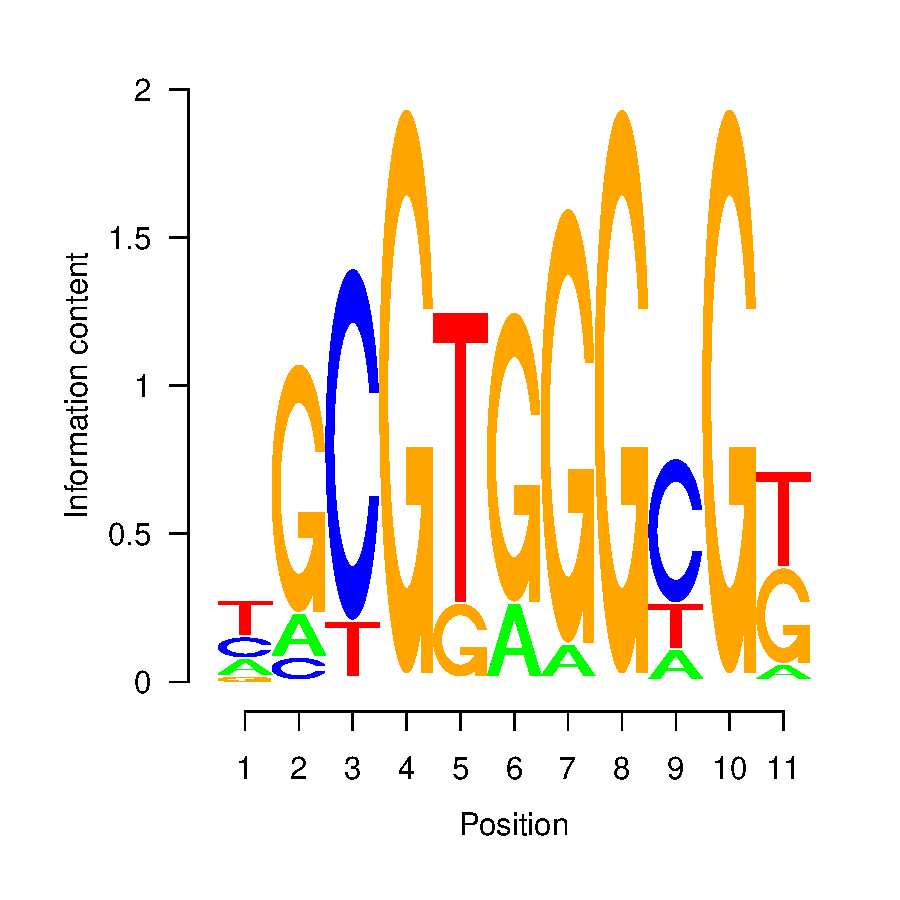
\includegraphics[width=0.3\textwidth]{MotifDb-egr1}
  \caption{Mmusculus-JASPAR\_CORE-Egr1-MA0162.1}
\end{figure}

\section{Motif Matching}
We will look for the ten position frequency matrices which are the best match to JASPAR's mouse EGR1, using
the MotIV package.  We actually request the top eleven hits from the entire MotifDb, since the first hit
should be the target matrix itself, since that is of necessity found in the full MotifDb.

\begin{Schunk}
\begin{Sinput}
> egr1.hits <- motifMatch (as.list (egr1.motif) [1], as.list (MotifDb), top=11)